\documentclass[10pt]{beamer}
% \usetheme{Warsaw}
% \usecolortheme{seagull}

\usepackage{amsthm}
\usepackage{ulem}
\usepackage{xcolor}
\usepackage{amsmath}
\usepackage{amssymb}
\usepackage{courier}
\usepackage{geometry}
\usepackage{enumitem}
\usepackage{graphicx}
\usepackage{listings}
\usepackage{algorithm}
\usepackage{algorithmic}
\usepackage{indentfirst}
\usepackage{verbatim}
\usepackage[perpage,stable]{footmisc}

\lstset{numbers=left, language=C++,basicstyle=\ttfamily\small,frame=shadowbox,
	keywordstyle=\color{blue!70}, commentstyle=\color{red!50!green!50!blue!50},
	escapeinside='',extendedchars=false}


\mode<presentation> {
  \usetheme{Boadilla}
  % or CambridgeUS, boxes, Warsaw, Madrid, many others
   \setbeamercovered{transparent}
  % or whatever (possibly just delete it)
  }

% \usepackage[english]{babel}
% \usepackage[latin1]{inputenc}
% \usepackage{times}
% \usepackage[T1]{fontenc}
% Or whatever. Note that the encoding and the font should match. If T1
% does not look nice, try deleting the line with the fontenc.

% \mode<handout>{
% \usepackage{pgfpages}
% \pgfpagesuselayout{4 on 1}[a4paper,landscape,border shrink=5mm]
% \setbeamercolor{background canvas}{bg=black!10} }

\linespread{1.4}

\definecolor{fgreen}{rgb}{0.1333,0.5451,0.1333}
\definecolor{dred}{rgb}{0.5451,0,0}

\newcommand{\tgreen}[1]{\textcolor{fgreen}{#1}}
\newcommand{\tred}[1]{\textcolor{dred}{#1}}
\newcommand{\itema}{\item[*]}

\AtBeginSection[]
  {
     \begin{frame}<beamer>
     \frametitle{Outline}
     \tableofcontents[currentsection]
     \end{frame}
  }

\begin{document}

	\title{6.172 Final Project}
	\author{Yinzhan Xu, Haoran Xu, Yuzhou Gu, Chengkai Zhang}
	\date{}

	\begin{frame}
		\titlepage
	\end{frame}

	\begin{frame}{Main results}

        \begin{table}
        \begin{minipage}[b]{0.45\textwidth}
        \centering
        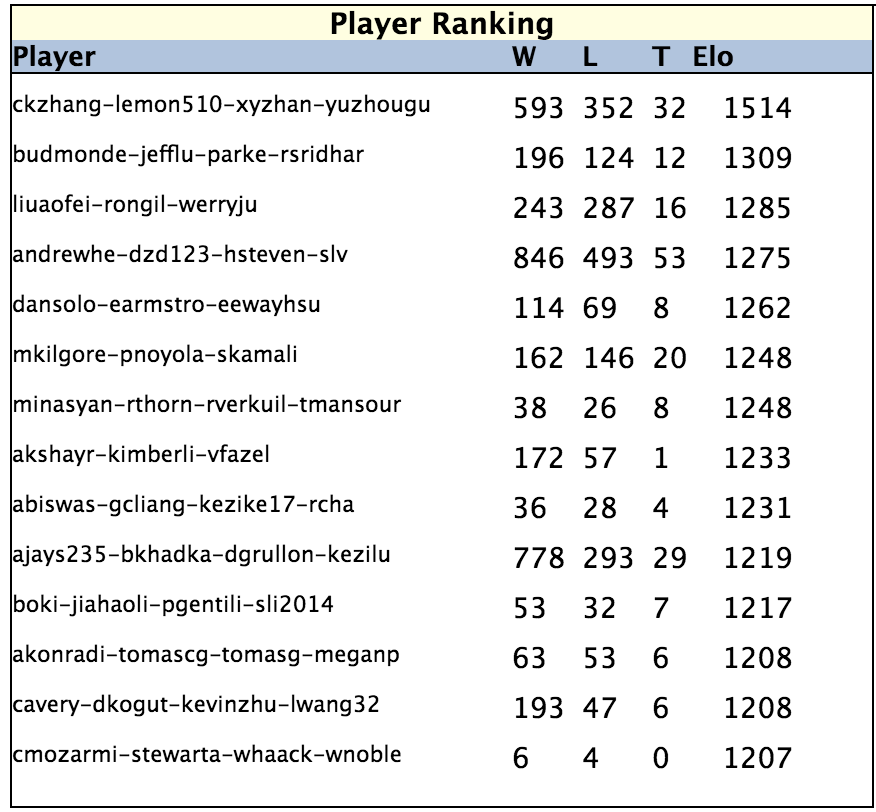
\includegraphics[width=0.9\textwidth]{scrimmage_old.png}

        Highest: 1514
        \end{minipage}
        % \hfill
        \begin{minipage}[b]{0.45\textwidth}
        \centering
        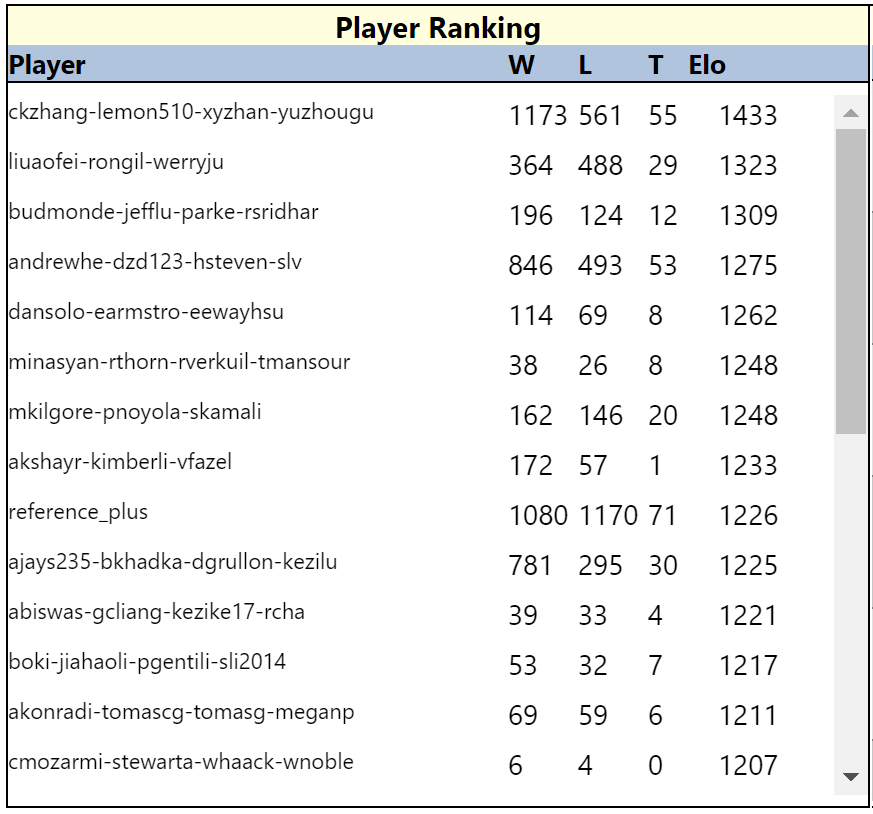
\includegraphics[width=0.9\textwidth]{scrimmage_current.png}

        Current: 1418
        \end{minipage}
        \end{table}
        \centering
        Average depth: Blitz: 7.6, Regular: 8.3


	\end{frame}

    \begin{frame}{Outline}
    \tableofcontents
    \end{frame}

%%%%%%%%%%%%%%%%%%%%%%%%%%%%%%%%%%%%%%%%%%%%%%%%%%%%%%%%%%%%%%%%%%%%%%%%%%%%%%%%%%%%%%%
    \section{Bottleneck Improvement}
    \begin{frame}{Bottleneck Improvement - \tt{scout\_search}}

        {\tt scout\_search} takes $32.55\%$ of the time and does the following:
        \begin{itemize}
            \itema Get a list of possible moves
            \itema Sort the moves
            \itema Check each move in order, do a recursive search if {\it necessary}
        \end{itemize}
    \end{frame}

	\begin{frame}{Bottleneck Improvement - \tt{scout\_search}}
	    \begin{itemize}
	        \itema Hash table move from pre-evaluation and killer moves are returned with high probability \\
	        $\Rightarrow$ check them first before generating move list
	        \itema A move is ignored if the node is quiescent and there is no victim\\
	        $\Rightarrow$ conservatively predict number of victims, exclude moves at quiescent node with no victim from move list
	        \itema About half of the moves have sort key of 0 \\
	        $\Rightarrow$ move them to end of move list directly and exclude from sorting procedure
	        \itema Maintaining node count introduces true sharing \\
	        $\Rightarrow$ remove counting
	    \end{itemize}


	\end{frame}
%%%%%%%%%%%%%%%%%%%%%%%%%%%%%%%%%%%%%%%%%%%%%%%%%%%%%%%%%%%%%%%%%%%%%%%%%%%%%%%%%%%%%%%
	\section{Openbook}
		\begin{frame}
		\frametitle{Motivation of Openbook}
		Underlying Assumption:
		\begin{itemize}
		\item[*] Good AI makes similar moves.
		\item[*] Possible good moves for a given game state are limited.
		\end{itemize}
		\pause
		Number of possible openings between two good AIs is reasonably small.

		Openbook!
	\end{frame}

	\begin{frame}
		\frametitle{Justification of Openbook}
		Validating the idea on real-world data:\pause
		\begin{itemize}
		\item[*] Downloaded the most recent 83000 games from Scrimmage.
		\item[*] Training Set: about 39000 games.
		\item[*] Test Set: about 44000 games.
		\pause
		\item[*] Consider the first \textcolor{dred}{5} rounds of game.
		\item[*] In Training Set, \textcolor{fgreen}{782 (2\%)} openings occurred at least \textcolor{fgreen}{twice}.
		\item[*] In Testing Set, \textcolor{fgreen}{2/3} of the openings falls into the 782 openings.
		\end{itemize}
		\pause
		Hits \textcolor{fgreen}{2/3} of the games with only \textcolor{fgreen}{782} records!
	\end{frame}

	\begin{frame}
		\frametitle{Advantage of Openbook}
		Openbook offers two main advantages:
		\begin{itemize}
		\item[*] We can search very deep for a good move in openbook.\\
		         So for the first several moves, our choice is very optimized.
		\item[*] And those moves take no time at all!
		\end{itemize}
		\pause
		If tested using default timing strategy:
		\begin{itemize}
		\item[*] Hitting \textcolor{fgreen}{5} rounds: \textcolor{fgreen}{20s} advantage in Regular, \textcolor{fgreen}{8s} advantage in Blitz.
		\item[*] Hitting \textcolor{fgreen}{10} rounds: \textcolor{fgreen}{38s} advantage in Regular, \textcolor{fgreen}{15s} advantage in Blitz.
		\end{itemize}
	\end{frame}

	\begin{frame}
		\frametitle{Calculating Openbook}
		Generating popular openings:
		\begin{itemize}
		\item[*] Used MySQL to manage data set for its convenience and power,
		and easiness to interact with web applications.
		\item[*] Downloaded the most recent 83000 games from Scrimmage.
		\item[*] Extracted frequent openings, and stored them into MySQL.
		\item[*] Search depth varied from \textcolor{fgreen}{9} to \textcolor{fgreen}{11} for each opening move.
		\item[*] Openings with higher \# of occurrences were calculated with deeper depth, for a possibly better move.
		\end{itemize}
	\end{frame}

	\begin{frame}
		\frametitle{Calculating Openbook}
		More than \textcolor{dred}{100000} openings generated.

		Impossible to calculate all of them with a single machine!\pause

		\textcolor{fgreen}{Distributed computing!}

		\begin{itemize}
		\item[*] LAMP (Linux+Apache+MySQL+PHP) web server to distribute down tasks and collect up results.
		\item[*] Clients use \tt{wget} to interact with web server.
		\item[*] \textcolor{fgreen}{150+} CPUs in Microsoft Azure.
		\item[*] \textcolor{fgreen}{15000+} CPU Hours in total.
		\end{itemize}
	\end{frame}

	\begin{frame}
		\frametitle{Calculating Openbook}

		Screenshot of our web server:

		\

		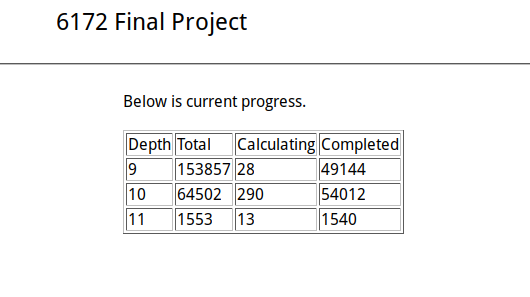
\includegraphics[scale=0.5]{screenshot1.png}
	\end{frame}

	\begin{frame}
		\frametitle{Openbook Test Results}

		\begin{itemize}
		\item Original Version: \textcolor{fgreen}{50\%} winrate against ReferencePlus.
		\item Openbook VS Original: \textcolor{fgreen}{61\%} winrate.\pause
		\item However..
		\item Openbook VS ReferencePlus: only \textcolor{dred}{45\%} winrate!
		\end{itemize}
	\end{frame}

	\begin{frame}
		\frametitle{Openbook Test Analysis}

		What might have happened?

		\begin{itemize}
		\item[*] The opening patterns of ReferencePlus are not captured in the data
		(at the time we capture data ReferencePlus is still not available).
		\item[*] A deeper search doesn't guaranteed a better move, but just gives a good move with higher probability.
		An unlucky bad move in the hotspot of openbook might actually degrade performance.
		\end{itemize}

		Experiments shows \textcolor{fgreen}{both} explanations are correct.
	\end{frame}

	\begin{frame}
		\frametitle{Boosting Openbook}

		Addressing the problem caused by missing opening patterns:

		\textcolor{fgreen}{Add the games played against ReferencePlus into Openbook!}

		\begin{itemize}
		\item[*] Before Boosting: \textcolor{dred}{45\%} winrate.
		\item[*] After Round 1 Boosting (1500 games): \textcolor{fgreen}{50\%} winrate.
		\item[*] After Round 2 Boosting (1500 games): \textcolor{fgreen}{56\%} winrate.
		\item[*] After Round 3 Boosting (1500 games): \textcolor{fgreen}{61\%} winrate.
		\end{itemize}

		Steady increase in winrate!
	\end{frame}

	\begin{frame}
		\frametitle{Boosting Openbook}

		Addressing the problem caused by popular bad move:

		The bot has a largely different winrate between moving first (\textcolor{dred}{30\%}) and moving second (\textcolor{fgreen}{60\%}).

		\begin{itemize}
		\item[*] Might the opening move ``h4g5'' actually be a bad move?
		\item[*] Rotate the King in the first move!
		\item[*] Now the game is very similar to as if we were moving second.
		\end{itemize}

		Amazing winrate increase: from \textcolor{dred}{45\%} to \textcolor{fgreen}{60\%}!

		Together with boosted openbook: \textcolor{fgreen}{69\%} winrate against ReferencePlus!
	\end{frame}

	\begin{frame}
		\frametitle{Openbook Summary}

		In the end, our openbook:
		\begin{itemize}
		\item[*] Contains about \textcolor{fgreen}{200000} game states arose from \textcolor{fgreen}{140000} games.
		\item[*] Almost always hits \textcolor{fgreen}{6} rounds.
		\item[*] With good probability hits \textcolor{fgreen}{7} or \textcolor{fgreen}{8} rounds.
		\item[*] Can sometime even reach \textcolor{fgreen}{10} rounds or more.
		\end{itemize}
	\end{frame}

	\begin{frame}
		\frametitle{Openbook Final Results against Refplus}

		\tred{remember to add in final result against refplus..}

	\end{frame}

%%%%%%%%%%%%%%%%%%%%%%%%%%%%%%%%%%%%%%%%%%%%%%%%%%%%%%%%%%%%%%%%%%%%%%%%%%%%%%%%%%%%%%%
	\section{Constant Optimization}
	\begin{frame}{Constant Optimization}
        \begin{itemize}
            \itema Use {\tt uint64\_t} to store cells that are lasered
            \itema Use two bitmaps to store occupied positions, one for each color
            \itema Change {\tt ARR\_SIZE} to 10
            \itema Precompute and use constant tables to save repeated computation in {\tt pcentral} and remove divisions
            \itema Pack {\tt victims\_t} in {\tt int16\_t} since storing all victims is unnecessary
            \itema Change the set in transposition table to be 4-way set-associative
        \end{itemize}
	\end{frame}


%%%%%%%%%%%%%%%%%%%%%%%%%%%%%%%%%%%%%%%%%%%%%%%%%%%%%%%%%%%%%%%%%%%%%%%%%%%%%%%%%%%%%%%
	\section{Strategies without performance gains}
	\begin{frame}{Strategies without performance gains}
	    \begin{itemize}
	        \itema Closebook: rarely used
	        \itema Range tree instead of sorting in  {\tt scout\_search}
	    \end{itemize}
	\end{frame}

\end{document}
